
\documentclass[10pt]{article}

\usepackage{graphicx,amsmath,amssymb,subfigure,enumerate,versions}
\usepackage{multicol,multirow,mdframed}
\usepackage{epstopdf}
\usepackage{pstricks,auto-pst-pdf}
\usepackage{pst-all}
\usepackage{pst-ode}
\usepackage{pst-math}
\usepackage{hyperref}
\usepackage{listings}
%\usepackage{mcode}
\lstset{language=Matlab}
\DeclareGraphicsExtensions{.png,.jpg,.pdf}

% ************ Page Margins *************
\hoffset=-1.3in
\setlength{\textwidth}{7.5in}
%%%%% MARGINS
\topmargin 0pt
\advance \topmargin by -\headheight
\advance \topmargin by -\headsep
\textheight 9.5in

% ************ Shortcuts *************
\newcommand{\Z}{\mbox{\sf Z\hspace{-1.5mm}Z}}
\newcommand{\SolutionSeparator}{ \hfill \hfill \hrule \hfill \hfill }
\newcommand{\R}{\mbox{\rm I\hspace{-0.75mm}R}}
\columnsep=0.75in
\newcommand{\vsc}{\vspace{1mm}}
\newcommand{\D}{\Delta }
\newcommand{\ifd}{f(x)~dx}
\newcommand{\dd}{\frac{dy}{dx} \,} 
\newcommand{\der}[2]{\frac{d{#1}}{d{#2}} \,}
\newcommand{\ddx}[1]{\frac{d {#1}}{dx} \,} 
\newcommand{\ddy}[1]{\frac{d {#1}}{dy} \,} 
\newcommand{\ddz}[1]{\frac{d {#1}}{dz} \,} 
\newcommand{\ddt}[1]{\frac{d {#1}}{dt} \,} 
\newcommand{\ds}{\displaystyle } 
\newcommand{\la}{\lambda } 
\newcommand{\del}{\nabla } 
\newcommand{\zx}{\frac{\partial z}{\partial x} \,}
\newcommand{\zy}{\frac{\partial z}{\partial y} \,}
\newcommand{\dx}{\frac{\partial f}{\partial x} \,}
\newcommand{\dy}{\frac{\partial f}{\partial y} \,}
\newcommand{\pp}[2]{\frac{\partial {#1}}{\partial {#2}} \,}
\newcommand{\ppx}{\frac{\partial }{\partial x} \,}
\newcommand{\ppy}{\frac{\partial }{\partial y} \,}
\renewcommand{\thesection}{\Roman{section}}
\newcommand{\vi}{\vec{i}}
\newcommand{\vj}{\vec{j}}
\newcommand{\vk}{\vec{k}}
\newcommand{\vv}{\vec{v}}
\newcommand{\lan}{\left\langle}
\newcommand{\ran}{\right\rangle}
\newcommand{\degr}{^{\circ}}

% *** Define the printed question style ***
\newcommand{\q}[1]{ {\em #1} }
% \renewcommand{\q}[1]{ {} }

\newcommand{\notice}{ \begin{center}Some problems and solutions
    selected or adapted from \\ Stewart {\em Calculus-Early
      Transcendentals} and Hughes-Hallett {\em Calculus} .\end{center}
}

% *** Overwrite, if desired, the question format
\includeversion{Question} 
\includeversion{Solution}

\newcommand{\multicolstart}{ }
\newcommand{\multicolend}{ }

\renewenvironment{Question}
{ \begin{mdframed}[nobreak=true,hidealllines=true,backgroundcolor=gray!50,innerleftmargin=5ex] }
{ \end{mdframed} }


% *** Footnoting with symbols ***
\long\def\symbolfootnote[#1]#2{\begingroup%
\def\thefootnote{\fnsymbol{footnote}}\footnote[#1]{#2}\endgroup}

\newcommand{\WeekTitleOne}{Derivatives - Foundations}
\newcommand{\WeekTitleTwo}{Derivatives - Linearization and Applications}
\newcommand{\WeekTitleThree}{Derivatives - Modeling}
\newcommand{\WeekTitleFour}{Integrals - Foundations}
\newcommand{\WeekTitleFive}{Integrals - Techniques}
\newcommand{\WeekTitleSix}{Integrals - Modeling}
\newcommand{\WeekTitleSeven}{Differential Equations - }
\newcommand{\WeekTitleEight}{Differential Equations - }
\newcommand{\WeekTitleNine}{Differential Equations - }
\newcommand{\WeekTitleTen}{Linear Algebra - }
\newcommand{\WeekTitleEleven}{Linear Algebra - }
\newcommand{\WeekTitleTwelve}{Linear Algebra - }


\begin{document}

\begin{center}
\subsection*{MNTC P01 - Week \#8 - \WeekTitleEight}
\end{center}

\begin{enumerate}

% ******************************
\item Use \verb@ode45@ to generate a graph of the solution to the
  following DEs, over the specified interval, given the initial
  condition.

\begin{enumerate}
\item $\ds \frac{dy}{dt} = t^2 + y^2$, $y(0) = 0$, and $0 \le t \le 1$.
\item $\ds \frac{dy}{dt} = \sin(t) + \cos(y)$, $y(0) = 0$, and $0 \le t \le 10$.
\item $\ds \frac{dy}{dt} = (1-y^2) + 0.2 \sin(t)$, $y(0) = 0$, and $0 \le t \le 20$.
\end{enumerate}


\begin{Solution}
Solutions are given in q\_ode45\_examples.m.
\end{Solution} 


% ******************************
\item Consider the single spring/mass system shown below:

\begin{center}
\includegraphics[width=3in]{Diagrams/Slide1}
\end{center}
where $\Fext$ is an external applied force.

Newton's second law gives us the relationship:
\begin{align*}
ma & = \sum F = \Fspring + \Fext \\
m \ddot{x} & = -k x + \Fext 
\end{align*}
where $k$ is the spring constant.

\begin{enumerate}
\item By hand, write this second order DE as a system of 1st order
  DEs, using the new variables $w_1 = x$ and $w_2 = \dot{x}$

\item Set $m =0.5$ kg, $k = 10$ N/m, and $\Fext$ to zero (no external
  force).  Define the differential equations in MATLAB in
  \verb#springDE.m#. Use \verb#ode45# to simulate the motion of the
  spring, given an initial displacement of $x(0) = 0.2$ m, and initial
  velocity of zero: $\dot{x}(0) = 0$.  Generate a plot with
\begin{itemize}
\item position against time (do {\em not} show the velocity), and
\item either choosing the time interval used for the \verb#ode45#
  simulation, or setting the graph's display limits on the graph with
  \verb#xlim#, to show the first 3 to 4 cycles only.
\end{itemize}

\item With the same initial conditions and constants as in (b),
  simulate the motion of the spring if we now apply an external force
  of $\Fext = \sin(t)$.  To do this, you will need to have to add both
  $t$ and $\Fext$ as arguments to the DE. e.g.
\begin{verbatim}
function dw_dt = springDE2(t, w, m, k, F_ext)
\end{verbatim}

  Generate a simulation over the time span $t = [0, 40]$ seconds, and
  plot the position against time.

  Explain why the motion looks so disorganized.

\item Repeat part (c), but with an external force of $\Fext = \sin(4
  t)$. Explain why the motion has cyclic waves in its amplitude.


\end{enumerate}

\begin{Solution}
\begin{enumerate}
\item  The first-order system would be:
\begin{align*}
\frac{d}{dt} w_1 & = \dot{x} = w_2 \\
\frac{d}{dt} w_2 & = \ddot{x} = \frac{1}{m} \left(-kx + \Fext\right) = \frac{1}{m} \left(-k w_1  + \Fext \right)
\end{align*}

\item The files ``springDE1.m'' and ``q\_springSimulation1.m'' generate
  this simulation.  In the plot, we see very nice example of harmonic
  motion.

\begin{center}
\includegraphics[width=3in]{q_springSimulation1}
\end{center}

\item The files ``springDE2.m'' and ``q\_springSimulation2.m'' generate
  this simulation.  In the plot, we see that the natural frequency and
  the regular stimulation by the outside force are quite out of step
  with each other, resulting in very disorganized motion.

\begin{center}
\includegraphics[width=3in]{q_springSimulation2}
\end{center}

\item The file ``q\_springSimulation3.m'' generates this simulation.
  In the plot, we see that the natural frequency and the regular
  stimulation by the outside force are close to each other (natural
  frequency is $\omega = \sqrt{\frac{10}{0.5}} \approx 4.5$, rad/s,
  and the stimulating frequency is at $\omega = 4$ rad/s.  This close
  match of the frequencies leads to the phenonenon called {\em beats}.

\begin{center}
\includegraphics[width=3in]{q_springSimulation3}
\end{center}


\end{enumerate}
\end{Solution}


% ******************** PENDULUM ********************************

\item In class, we saw the differential equation for the angular
  motion of a pendulum.  Here it is again, with no friction.
\begin{align*}
  \mbox{Newton's Second Law: }   m  L^2 \theta'' & = T_g \\
  & = - m L g \sin(\theta)  \\
  \mbox{Solving for $\theta''$: }\theta'' & = - \frac{g}{L} \sin(\theta) 
\end{align*}

Without simulating the actual motion of the pendulum, we can compute
the period, $T$, using the formula below:
\begin{align*}
  T = 4 \sqrt{L/g} \int_0^{\pi/2} \frac{dx}{\sqrt{1 - k^2 \sin^2 x}}
\end{align*}
where $k = \sin\left(\frac{1}{2} \theta_0\right)$ and $g$ is the
acceleration due to gravity, $9.8 $ m/s.  


For each set of values for $L$ and $\theta_0$,
\begin{enumerate}[(a)]
\item Use \verb#quad# to find the period of the pendulum oscillations,
  and
\item confirm the period by using \verb#ode45# to simulate the motion
  pendulum for exactly that length of time, and plot a graph of the
  angular {\bf velocity} against time.  The velocity should just reach
  zero at the end of one cycle.
\end{enumerate}

\begin{enumerate}[(i)]
\item $L = 2$ m, $\theta_0 = 40^o$, 
\item $L =2.5$ m, $\theta_0 = 20^o$.
\item $L =5.0$ m, $\theta_0 = 90^o$.
\end{enumerate}

\begin{solutions}

  All of the problems are shown solved in \verb#q_pendulum.m#.

  \begin{enumerate}[(i)]
  \item $L = 2$ m, $\theta_0 = 40^o$:  {\bf T = 2.9274}
  \item $L =2.5$ m, $\theta_0 = 20^o$: {\bf T = 3.1978}
  \item $L =5.0$ m, $\theta_0 = 90^o$: {\bf T = 5.2974}
  \end{enumerate}

Plots: \\
\includegraphics[width=2in]{q_pendulum_1} 
\includegraphics[width=2in]{q_pendulum_2} 
\includegraphics[width=2in]{q_pendulum_3} 

\end{solutions}




% ******************** Newton's Cooling  ********************************
\item Newton's law of heating and cooling states that an object with
  temperature $T$ in an environment at temperature $T_{ext}$ will heat
  up or cool down according to the differential equation

 $$\frac{dT}{dt} = -k (T - T_{ext})$$

 Consider a garage used as a workshop.  Its insulation and surface
 area give $k$ a value of 0.1, if time $t$ is measured in hours and
 the temperatures, $T$ and $T_{ext}$, are in degrees Celsius.

The temperature outside changes during the day, as described by
the formula 
$$T_{ext} =  10 + 7 \cos\left(\frac{\pi}{12} t\right)$$

We now imagine that the power goes out, with the garage at 23$^o$ C at
$t=0$.

\begin{enumerate}
\item Use ode45 and the DE to generate a numerical prediction of the
  garage's temperature $T$ over time.  Graph the solution over a time
  interval that shows both the initial and long-term behaviour of the
  temperature.

  For the following questions, just use the graph or the numerical
  prediction of the temperature. You are {\em not} expected to solve
  the DE analytically.

\item How many days does it take for the garage to get into a
  consistent temperature cycle?  (You will need to estimate this by
  eye.)

\item How many degrees does the temperature in the building fluctuate
  by, once the temperature gets into a steady cycle?

\item Suppose the building were better insulated, so that the rate of
  heat loss were cut in half.  Should $k$ be half as large, or twice
  as large?  

\item Generate a numerical prediction for the temperature over time in
  the better-insulated scenario, and produce a graph of the
  temperature vs time for both scenarios on the same axes.
  
\item How large are the temperature fluctuations in the building, now
  that the extra insulation has been added?  Does halving the net heat
  flow also halve the net temperature fluctuations?
\end{enumerate}

\begin{solutions}\begin{solution}
\begin{enumerate}
\item  A graph of the temperature over time is shown below: 
  
 \includegraphics[width=3in]{GraphQ3_1a}

 MATLAB code is available in \verb#q_garageTemp.m#

\item From the graph, it takes the building roughly 2 days (48 hours)
  to get into a repeating cycle of temperature variation.

\item Careful zooming of the graph (or a look at the $y$ values in the
  ode45 output) give a highest temperature of 12.5 (high) and 7.5
  (low), for a net fluctuation of approximately 2.6 degrees per day.

\item $k$ represents the coefficient of heat flow between the building
  and the environment. The bigger $k$ is, the {\em larger} the
  headflow between the two.  Since we're adding insulation, this
  should {\em reduce} the heat flow, and so {\em lower} the value of
  $k$.

\item A graph of the heat change over time, given better insulation,
  is shown below.

  \includegraphics[width=3in]{GraphQ3_1a_insulated}

\item Zooming in on the peaks of the graph, the temperature now
  fluctuates between approximately 11.3 and 8.8 degrees Celsius, for a
  range of 2.5 degrees.  This {\em is} roughly half the magnitude of
  the fluctuations we saw earlier.

\end{enumerate}
\end{solution}
\end{solutions}
% ******************************
\item 
\begin{Question} %9.1 - 1
  Show that $\ds y = \frac{2}{3}\text{e}^{x} + \text{e}^{-2x}$ is a solution of the differential equation $y' + 2y = 2\text{e}^{x}$. \\
\end{Question}

% 1 - Solution
\begin{Solution}
\begin{equation*}
y = \frac{2}{3}\text{e}^{x} + \text{e}^{-2x} \Rightarrow
y' = \frac{2}{3}\text{e}^{x} - 2\text{e}^{-2x}
\end{equation*}
To show that $y$ is a solution of the differential equation, we will substitute the expressions for $y$ and $y'$ in the left-hand side of the equation and show that the left-hand side of the equation and show that the left-hand side is equal to the right-hand side.

\begin{align*}
	\text{LHS} &= y' + 2y = \frac{2}{3}\text{e}^{x} - 2\text{e}^{-2x} + 2(\frac{2}{3}\text{e}^{x} + \text{e}^{-2x}) \\
	&= \frac{2}{3}\text{e}^{x} - 2\text{e}^{-2x} + 
	\frac{4}{3}\text{e}^{x} + 2\text{e}^{-2x} =
	\frac{6}{3}\text{e}^{x} = 2\text{e}^{x} \\ 
	&= \text{RHS}
\end{align*}
\end{Solution}
%%%%%%%%%%%%%%%%%%

%9.1 - 3
\item
\begin{Question}
\begin{enumerate}[(a)]
\item For what values of $r$ does the function $y = \text{e}^{rx}$ satisfy the differential equation $2y'' + y' - y = 0$?

\item If $r_1$ and $r_2$ are the values of $r$ that you found in part (a), show that every member of the family of functions $y = a\text{e}^{r_{1}x} + b\text{e}^{r_{2}x}$ is also a solution.
\end{enumerate}
\end{Question}

\begin{Solution}
\begin{enumerate}[(a)]
\item \begin{equation*}
		y = \text{e}^{rx} \Rightarrow
		y' = r\text{e}^{rx} \Rightarrow
		y'' = r^2\text{e}^{rx}
	\end{equation*}
	Substituting these expressions into the differential equation 
	$2y'' + y' - y = 0$, we get
	\begin{align*}
		&2r^2\text{e}^{rx} + r\text{e}^{rx} - \text{e}^{rx} = 0 \\
		\Rightarrow \quad &(2r^2 + r - 1)\text{e}^{rx} = 0 \\
		\Rightarrow \quad &(2r - 1)(r + 1) = 0
	\end{align*}
	(since $\text{e}^{rx}$ is never zero) $r = \frac{1}{2}$ or -1.

\item Let $r_1 = \frac{1}{2}$ and $r_2 = -1$, so we need to show that every member of the family of functions $y = a\text{e}^{x/2} + b\text{e}^{-x}$ is a solution of the differential equation $2y'' + y' - y = 0$.\\
\begin{align*}
	&y = a\text{e}^{x/2} + b\text{e}^{-x} \\
	\Rightarrow \quad &y' = \frac{1}{2}a\text{e}^{x/2} - b\text{e}^{-x}\\
	\Rightarrow \quad &y'' = \frac{1}{4}a\text{e}^{x/2} + b\text{e}^{-x}
\end{align*}
\begin{align*}
	\text{LHS} &= 2y'' + y' - y \\ 
	&= 2(\frac{1}{4}a\text{e}^{x/2} + b\text{e}^{-x}) + (\frac{1}{2}a\text{e}^{x/2} - b\text{e}^{-x}) \\ & \hspace{4mm}- (a\text{e}^{x/2} + b\text{e}^{-x}) \\
	&= \frac{1}{2}a\text{e}^{x/2} + 2b\text{e}^{-x} + \frac{1}{2}a\text{e}^{x/2} - b\text{e}^{-x}  \\
	& \hspace{4mm}- a\text{e}^{x/2} - b\text{e}^{-x} \\
	&= (\frac{1}{2}a + \frac{1}{2}a - a)\text{e}^{x/2} + (2b - b -b)\text{e}^{-x} \\
	&= 0 \\ &= \text{RHS}
\end{align*}
\end{enumerate}
\end{Solution}
%%%%%%%%%%%%%%%%%%

%9.1 - 4
\item
\begin{Question}
\begin{enumerate}[(a)]
\item For what values of $k$ does the function $y = \cos(kt)$ satisfy
  the differential equation $4y'' = -25y$?
\item For those values of $k$, verify that every member of the vamily of functions $y = A\sin kt + B\cos kt$ is also a solution.
\end{enumerate}
\end{Question}

\begin{Solution}
\begin{enumerate}[(a)]
\item \begin{equation*}
		y = \cos kt \ \Rightarrow \ y' = -k \sin kt \ \Rightarrow \ y'' = -k^2 \cos kt
	\end{equation*}
	Substituting expressions into the differential equation $4y'' = -25y$, we get 
	\begin{align*}
		&4(-k^2\cos kt) = -25(\cos kt) \\
		\Rightarrow \quad &(25 - 4k^2) \cos kt = 0 (\text{for all } t)\\
		\Rightarrow \quad &25 - 4k^2 = 0 \\
		\Rightarrow \quad &k^2 = \frac{25}{4} \ \Rightarrow \ k = \pm \frac{5}{2}
	\end{align*}
	
\item \begin{align*}
		&y = A\sin kt + B \cos kt \\
		\Rightarrow \quad &y' = Ak\cos kt - Bk \sin kt \\
		\Rightarrow \quad &y'' = -Ak^2 \sin kt - Bk^2 \cos kt
	\end{align*}
	The given differential equation $4y'' = -25y$ is equivalent to $4y'' + 25y = 0$.  Thus,
\begin{align*}
	\text{LHS} &= 4y'' + 25y \\
	&= 4(-Ak^2 \sin kt - Bk^2 \cos kt) \\
	& \quad + 25(A\sin kt + B\cos kt) \\
	&= -4Ak^2 \sin kt - 4Bk^2 \cos kt \\
	& \quad+ 25A\sin kt + 25B \cos kt \\
	&= (25 - 4k^2)A\sin kt + (25 - 4k^2)B\cos kt \\
	&= 0 \hspace{4mm} \text{since } k^2 = \frac{25}{4}
\end{align*}
\end{enumerate}
\end{Solution}
%%%%%%%%%%%%%%%%%%

%9.1 - 7
\item
\begin{Question}
\begin{enumerate}[(a)]
\item What can you say about a solution of the equation $y' = -y^2$ just by looking at the differential equation?
\item Verify that all members of the family $y = 1/(x + C)$ are solutions of the equation in part (a).
\item Can you think of a (very simple) solution of the differential
  equation $y' = -y^2$ that is not a member of the family in part (b)?
\item Find the solution to the initial-value problem
\begin{equation*}
	y' = -y^2 \hspace{6mm} y(0) = 0.5
\end{equation*}
\end{enumerate}
\end{Question}
\begin{Solution}
\begin{enumerate}[(a)]
\item Since the derivative of $y' = -y^2$ is always negative (or 0 if $y = 0$), the function $y$ must be decreasing (or equal to 0) on any interval on which it is defined.
\item $y = \frac{1}{x + C} \Rightarrow y' = -\frac{1}{(x + C)^2}$.\\
$\text{LHS} = y' = -\frac{1}{(x + C)^2} = -\left(\frac{1}{x + C} \right)^2 = -y^2 = \text{RHS}$
\item $y=0$ is a solution of $y'=-y^2$ that is not a member of the family in part (b).
\item If $y(x) = \frac{1}{x + C}$, then $y(0) = \frac{1}{0 + C} = \frac{1}{C}$.  Since $y(0) = 0.5$, $\frac{1}{C} \frac{1}{2} \Rightarrow C = 2$, so $y =\frac{1}{x + 2}$
\end{enumerate}
\end{Solution}
%%%%%%%%%%%%%%%%%%

\hrulefill

\subsection*{Numerical ODE Solutions With MATLAB}


%*******************************
\item
\begin{Question}
  Create a plot for the solution to the differential equation
  $y' - \frac{y^2}{x^3} = 0$ if y(2) = 1.  Include a large enough
  \verb#xspan# to see the long-term behaviour.
\end{Question}

\begin{Solution}
  For this first example of use MATLAB to build a numerical solution
  to a DE, we will show the full listing of a script that generates a
  solution to the given differential equation.  In later solutions, we
  will only include the key lines for the MATLAB script.

  Notes: 
  \begin{itemize}
  \item We set \verb#xspan# to start at 2 in the line
    \verb#xspan = [2, 30]#.  This is used because the solution MATLAB
    is generating will start at the coordinates $x_0$ = first element
    of \verb#xspan#, and $y_0$ = \verb#y0# in the code, and our
    initial condition is $x = 2$, $y=1$.
  \item We find the second value in the time span with some trial and
    error.  Any value larger than 15 or 20 would be sufficient to show
    the long-term trend in the solution.
  \end{itemize}
\lstinputlisting[showstringspaces=false]{MATLAB/W07DE01.m}

Link to the MATLAB code: \\
\href{http://www.mast.queensu.ca/~apsc171/MNTCP01/PracticeProblems/MATLAB/W07DE01.m}{W07DE01.m}

Here is the graph of the solution.

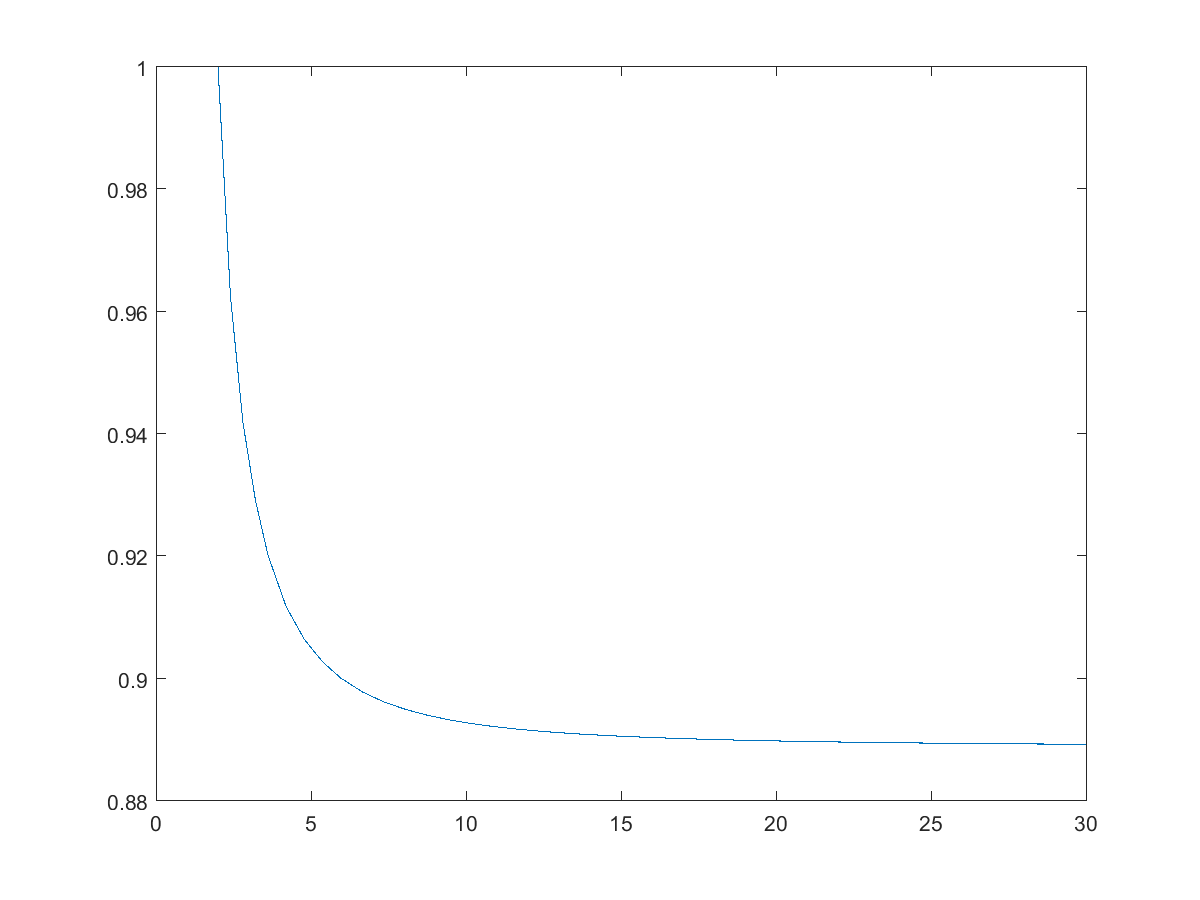
\includegraphics[width = 0.5\linewidth]{graphics/Week07_DESolutions/W07DE01}

    
\end{Solution}


%*******************************
\item
\begin{Question}
Create a plot for the solution to the differential equation
  $(2y - 4)y' - 3x^2 = 4x - 4$, if y(1) = 3.
    
\end{Question}

\begin{Solution}
  To generate a first-order DE solution in MATLAB, the differential
  equation must be written first in the form $y' = \ldots$.
  \begin{align*}
    (2y - 4)y' - 3x^2 & = 4x - 4 \\
    (2y - 4)y' & =  3x^2 +4x - 4 \\
    y' & =  \frac{(3x^2 +4x - 4)}{(2y - 4)} \\
  \end{align*}
    
Link to the MATLAB code: \\
\href{http://www.mast.queensu.ca/~apsc171/MNTCP01/PracticeProblems/MATLAB/W07DE02.m}{W07DE02.m}

Here is the graph of the solution.

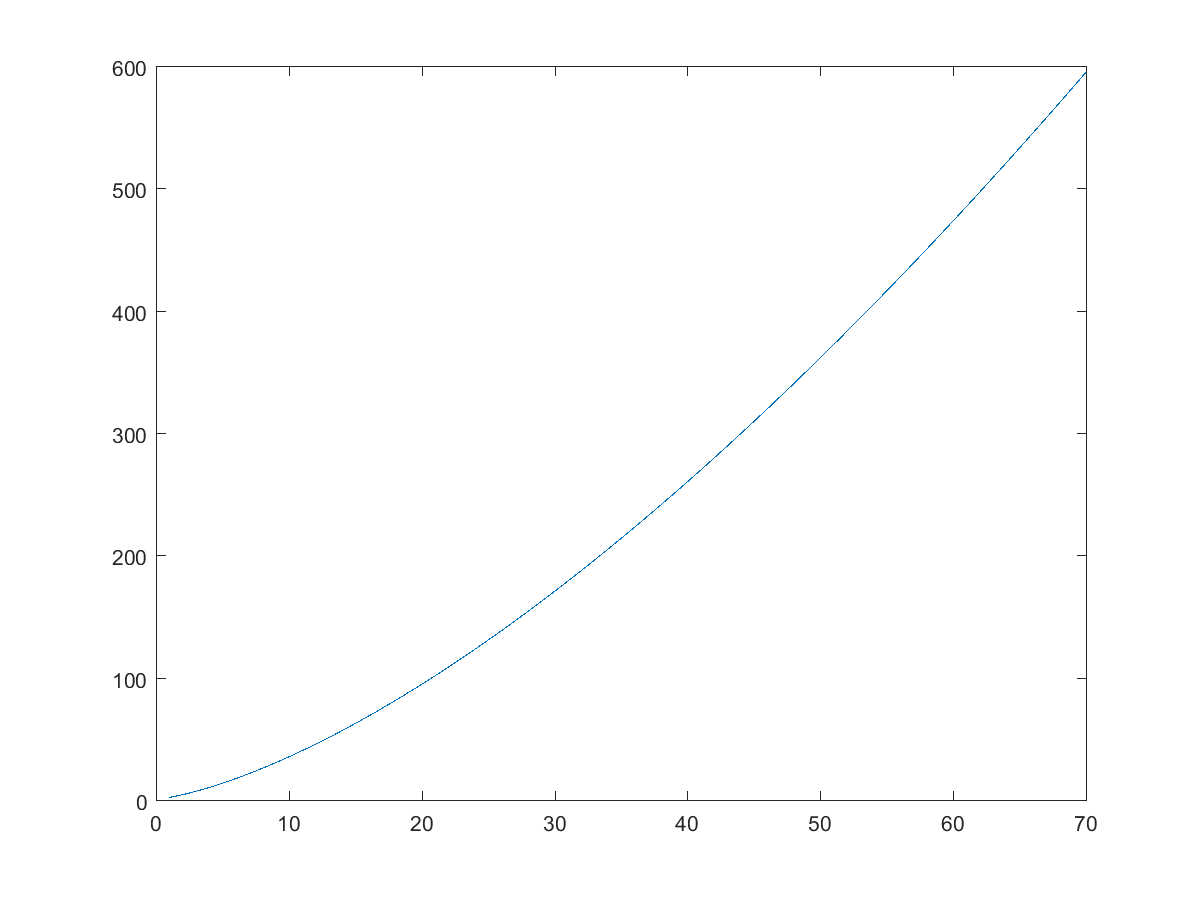
\includegraphics[width = 0.5\linewidth]{graphics/Week07_DESolutions/W07DE02}
\end{Solution}


%*******************************
\item
\begin{Question}
Create a plot for the solution to the differential equation
  $y' = e^{-y}(2t - 4)$ if $y(0) = 5$
    
\end{Question}

\begin{Solution}
  This DE is already in the form $y' = \ldots$, so we can input it
  into MATLAB as-is.  Note that the independent variable in this
  example is $t$, so we will use that in MATLAB instead of the
  variable $x$.


Link to the MATLAB code: \\
\href{http://www.mast.queensu.ca/~apsc171/MNTCP01/PracticeProblems/MATLAB/W07DE03.m}{W07DE03.m}

Here is the graph of the solution.

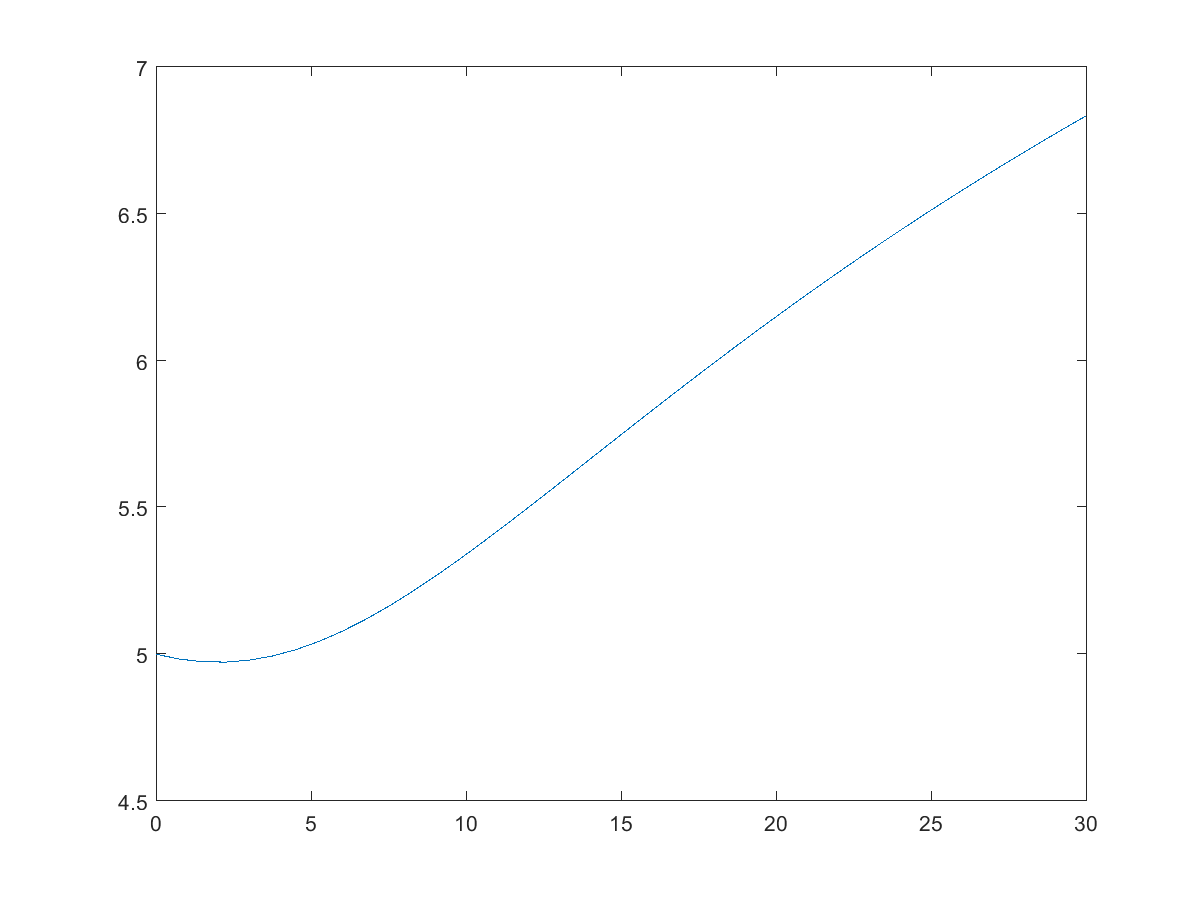
\includegraphics[width = 0.5\linewidth]{graphics/Week07_DESolutions/W07DE03}


    
\end{Solution}

%*******************************
\item
\begin{Question}
Create a plot for the solution to the differential equation
  $ty' - 2y = t^5 \sin (2t) - t^3 + 4t^4$, if
  $y(\pi) = \frac{3}{2}\pi^4$
    
\end{Question}

\begin{Solution}
  To generate a first-order DE solution in MATLAB, the differential
  equation must be written first in the form $y' = \ldots$.
  \begin{align*}
    ty' - 2y & = t^5 \sin (2t) - t^3 + 4t^4 \\
    ty' & = 2y + t^5 \sin(2t) - t^3 + 4t^4 \\
    y' & = \frac{1}{t} (2y + t^5 \sin(2t) - t^3 + 4t^4) \\
  \end{align*}
    
Link to the MATLAB code: \\
\href{http://www.mast.queensu.ca/~apsc171/MNTCP01/PracticeProblems/MATLAB/W07DE04.m}{W07DE04.m}

Here is the graph of the solution.

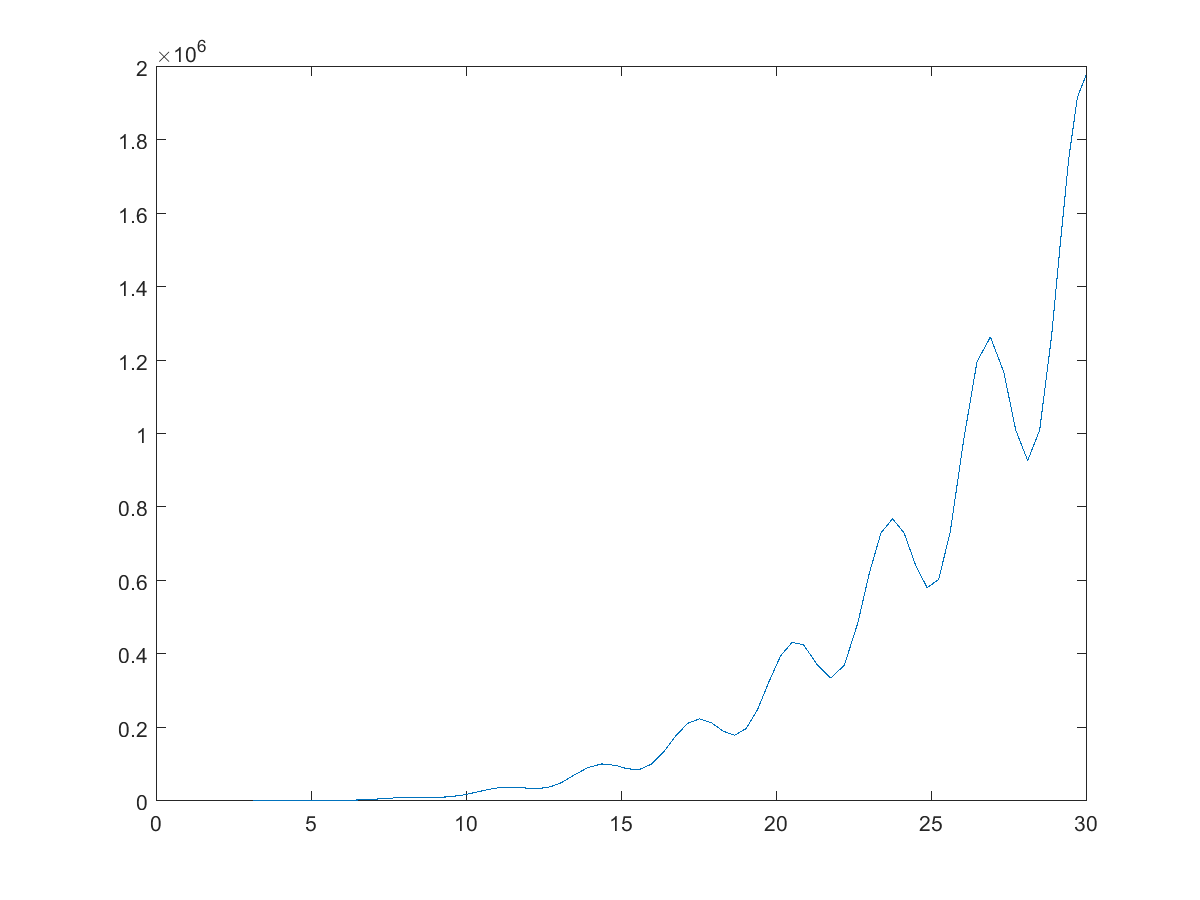
\includegraphics[width = 0.5\linewidth]{graphics/Week07_DESolutions/W07DE04}
    
Note that in this example, because of the $\sin(2t)$ introducing an
oscillation in the system, the solution won't look at simple as some
of the other examples.
\end{Solution}

%*******************************
\item
\begin{Question}
  Create a plot for the solution to the differential equation
  $ty' + 2y = t^2 - t + 1$, if $y(1) = 0.5$.
    
\end{Question}

\begin{Solution}
  To generate a first-order DE solution in MATLAB, the differential
  equation must be written first in the form $y' = \ldots$.
  \begin{align*}
    ty' + 2y = t^2 - t + 1 \\
    ty' = -2y + t^2 - t + 1 \\
    y' = \frac{1}{t} (-2y + t^2 - t + 1) \\
  \end{align*}
    
Link to the MATLAB code: \\
\href{http://www.mast.queensu.ca/~apsc171/MNTCP01/PracticeProblems/MATLAB/W07DE05.m}{W07DE05.m}

Here is the graph of the solution.

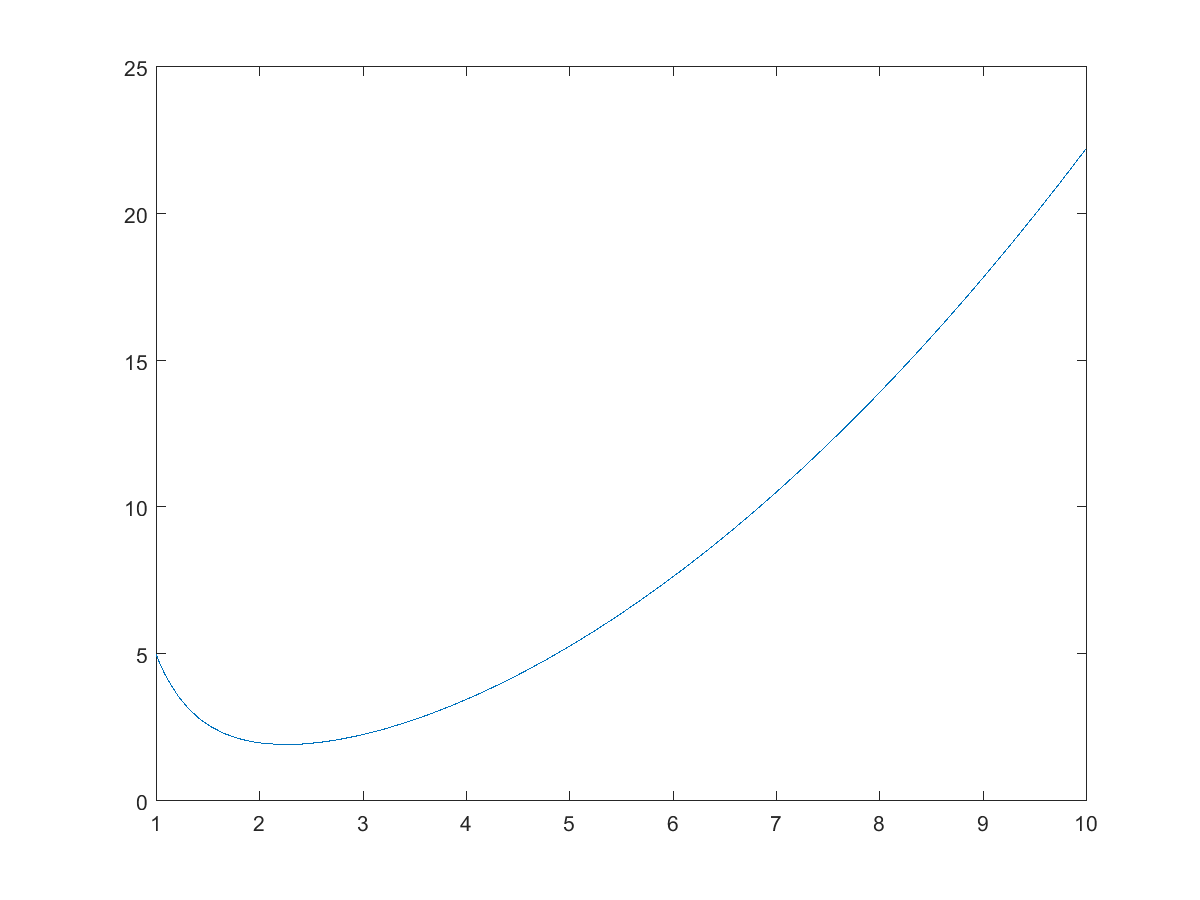
\includegraphics[width = 0.5\linewidth]{graphics/Week07_DESolutions/W07DE05}
    
    
\end{Solution}

%*******************************
\item
\begin{Question}
  Create a plot for the solution to the differential equation
  $2xy^2 + 4 = 2(3 - x^2y)y'$ if $y(5) = 8$.
    
\end{Question}

\begin{Solution}
  To generate a first-order DE solution in MATLAB, the differential
  equation must be written first in the form $y' = \ldots$.  We start
  by switching both sides of the equation to put $y'$ on the left.
  \begin{align*}
    2(3 - x^2y)y' & = 2xy^2 + 4   \\
    y' & = \frac{ 2xy^2 + 4}{2 (3-x^2 y)} 
  \end{align*}
    
Link to the MATLAB code: \\
\href{http://www.mast.queensu.ca/~apsc171/MNTCP01/PracticeProblems/MATLAB/W07DE06.m}{W07DE06.m}

Here is the graph of the solution.

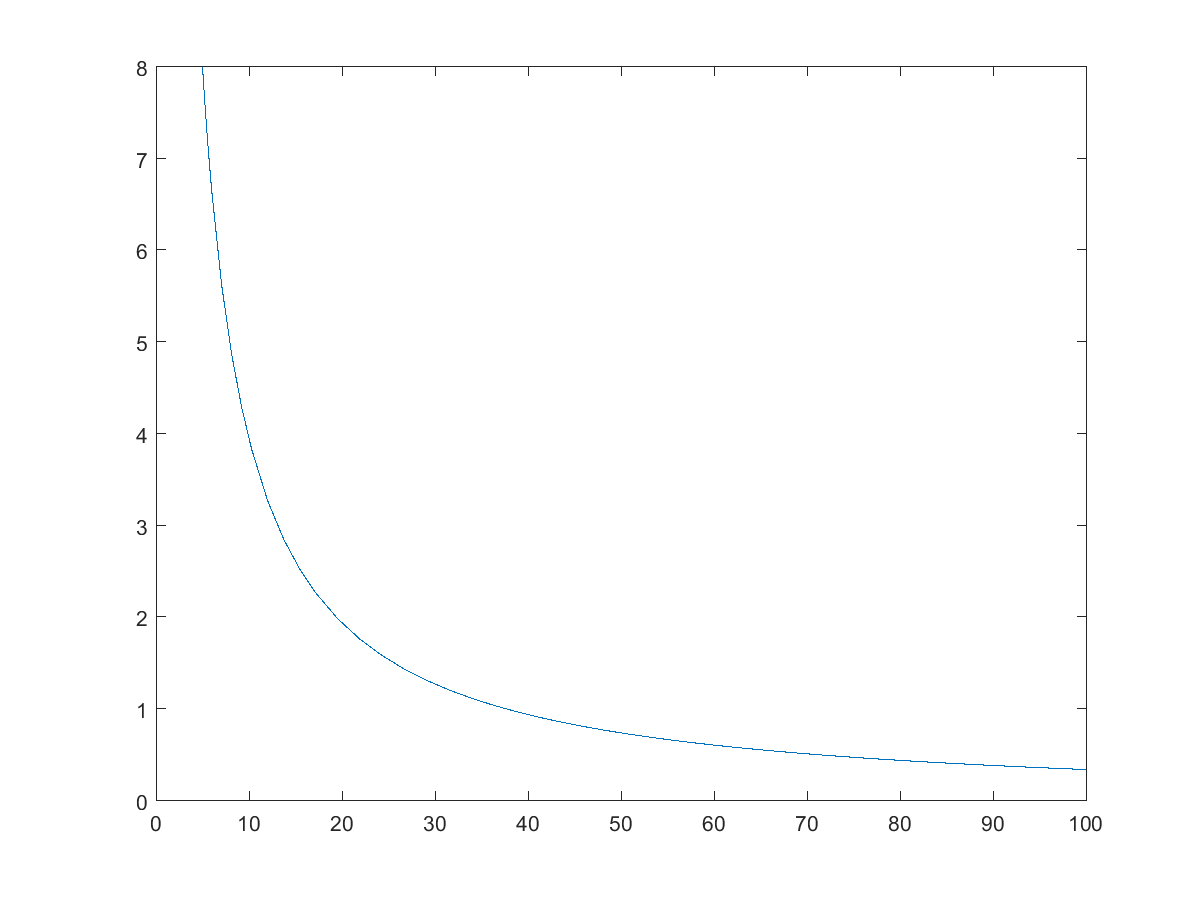
\includegraphics[width = 0.5\linewidth]{graphics/Week07_DESolutions/W07DE06}
    
    
\end{Solution}

%****************
\item 
\begin{Question}
Find the particular solution to the IVP 
$y'' + 4y = 2x$, $y(0)=1$, $y'(0) = 2$.

\end{Question}

\begin{Solution}

$y_c = c_1 \cos(2x) + c_2 \sin(2x)$

$y_p = A + Bx$ \\
$y'_p = B$ \\
$y''_p = 0$ \\

Substituting into the DE gives $A = \frac{1}{2}$ and $B = 0$, so the
general solution is
$$ y = y_c + y_p = c_1 \cos(2x) + c_2 \sin(2x) + \frac{x}{2}$$

To find $c_1$ and $c_2$, use the initial conditions:
\begin{align*}
  y(0) = 1: ~~~~~ 1 & = c_1 + 0 + 0 \\
  y'(0) = 2: ~~~~~ 2 & = 0 +  2c_2   + \frac{1}{2} \\
\end{align*}
Solving gives
$$ y =  1 \cdot \cos(2x) + \frac{3}{4} \sin(2x) + \frac{x}{2}$$

\end{Solution}

\item 
  \begin{Question}
    Find the particular solution to the IVP $ y'' + 9 y = \sin(2x)$,
    $y(0)=1$, $y'(0)=0$.
  \end{Question}

 \begin{Solution}
$y_c = c_1 \cos(3x)  c_2 \sin(3x)$

$y_p = A \cos(2x) + B \sin(2x)$.  Solving for $A$ and $B$ gives $A =
0$ and $B = \frac{1}{5}$.  The general solution is

$$y = c_1 \cos(3x) + c_2 \sin(3x) + \frac{1}{5} \sin(2x)$$

Using the initial conditions, we can solve for $c_1 = 1$ and $c_2 = -\frac{2}{15}$

$$ y = \cos(3x) - \frac{2}{15}\sin(3x) + \frac{1}{5} \sin(2x)$$
 \end{Solution}
\subsection*{Applications}

%****************
\item 
\begin{Question}
For a spring/mass system with $m=1$ kg, $c=6$ N/(m/s), and
  $k=45$, approximately what frequency of external forcing would
  produce the largest amplitude steady-state vibration?
\end{Question}

\begin{Solution}
  The natural frequency is found using the auxiliary equation $r^2 +
  6r + 45 = 0$, giving $r=-3 \pm 6i$, so $x_c = c_1 e^{-3t}\cos(6t) +
  c_2 e^{-3t} \sin(6t)$

Since this system's natural or intrinsic oscillations are at 6 rad/s,
the spring/mass will show the largest amplitude response to an outside
force if that outside force also has a frequency close to 6 rad/s.

\end{Solution}

%****************
\item 
\begin{Question}
For a spring/mass system with $m=1$ kg, $c=10$ N/(m/s), and
  $k=650$, approximately what frequency of external forcing would
  produce the largest amplitude steady-state vibration?
\end{Question}

\begin{Solution}
$m=1, c=10,k=650,F_0=100$, so
$$x'' + 10x' + 650x = \cos(\omega t)$$ 

The natural frequency is found using the auxiliary equation $r^2 + 10r
+ 650 = 0$, giving $r=-5 \pm 25i$, so $x_c = c_1 e^{-5t}\cos(25t) +
c_2 e^{-5t} \sin(25t)$

It will show its largest amplitude response to stimuli with
frequencies close to 25 rad/s.
\end{Solution}

%**********  
\item \begin{Question}
Consider the undamped spring model $y'' + \omega_0^2 y = \cos(\omega t)$.
    \begin{enumerate}
    \item Solve $y'' + \omega_0^2 y = \cos(\omega t)$ where $\omega^2
      \neq \omega_0^2$.
    \item What does this predict will happen to the amplitude of the
      oscillations as the stimulus frequence $\omega$ is brought
      closer and closer to the natural frequency $\omega_0$?
    \end{enumerate}
\end{Question}

\begin{Solution}
  \begin{enumerate}[(a)]
  \item 
  The characteristic equation is $r^2+ \omega_0^2 = \bigl( r - \omega_0
  \sqrt{-1}\bigr) \bigl( r + \omega_0 \sqrt{-1}\bigr)$, so the general solution
  to the corresponding homogeneous equation is $C_1 \cos( \omega_0 t) + C_2
  \sin(\omega_0 t)$.  Using the method of undetermined coefficients, we consider
  a solution of the form $y_g(t) := A_1 \cos(\omega t) + A_2 \sin(\omega t)$ for
  some constants $A_1$ and $A_2$.  It follows that
  \begin{align*}
    \cos(\omega t) &= y_g'' + \omega_0^2 y_g = \bigl( - A_1 \omega^2 \cos(\omega
    t) - A_2 \omega^2 \sin( \omega t) \bigr) + \omega_0^2
    \bigl(A_1 \cos(\omega t) + A_2 \sin(\omega t) \bigr) \\
    &= (\omega_0^2-\omega^2) \bigl( A_1 \cos(\omega t) + A_2 \sin(\omega t)
    \bigr)
  \end{align*}
  Since $\ds A_1 = \tfrac{1}{\omega_0^2 -\omega^2}$ and $A_2 = 0$, the general
  solution is 
  \[
  C_1 \cos( \omega_0 t) + C_2 \sin(\omega_0 t) + \frac{1}{(\omega_0^2
  -\omega^2)}\cos(\omega t) \, . \qedhere
  \]
\item As the stimulus frequency $\omega$ approaches the natural
  frequency $\omega_0$, the amplitude given by $\frac{1}{(\omega_0^2 -
    \omega^2)} \to \infty$.  This corresponds to the result of
  resonance, when $\omega = \omega_0$, and the solutions change to
  $y_c = A t \cos(\omega t)$, which has an linearly growing
  (unbounded) amplitude.
  \end{enumerate}
\end{Solution}
  \vspace*{0.5em}

%****************
\item 
  \begin{Question} 
Consider the equation for the spring/mass system
    with $m=1$ kg, $c=4$ N/(m/s) and $k = 4$ N/m, and which is being
    forced by an external periodic force of $10 \cos(3t)$ N: $$x'' +
    4x' + 4x = 10 \cos(3t)$$ Find the formula for the steady-state
    oscillations, and find their amplitude.
\end{Question}

\begin{Solution}
  The system is damped, so the $x_c$ solution will have negative
  exponentials in it. i.e. that part of the solution will be {\bf
    transient} because its contribution $\to 0$ over time.  That is
  why $x_c$ is referred to as $x_{\mbox{transient}}$ or
  $x_{\mbox{tr}}$ throughout the problems in this section.

  Since the RHS is pure cos/sine, its differential family will not
  overlap with the exp sin/cos in $x_c$.  This means $x_p$ will be a
  simple linear combination of $\cos(3t)$ and $\sin(3t)$.

Let $x_p = A \cos(3t) + B \sin(3t)$. \\
$x_p' = -3A \sin(3t) + 3B \cos(3t)$ \\
$x_p'' = -9A \cos(3t) - 9B \sin(3t)$ \\

Substituting into the DE,
$$ ( -9A \cos(3t) - 9B \sin(3t))
+4( -3A \sin(3t) + 3B \cos(3t))
+4(A \cos(3t) + B \sin(3t))  = 10 \cos(3t)$$ 
\begin{align*}
\mbox{sine coeffs: ~~~} -9B-12A+4B & = 0 & -12A -5B &= 0 \\
\mbox{cos coeffs: ~~~} -9A+12B+4A & = 10 & -5A + 12B &= 10\\
\\
-60A -25B & = 0 \\
-60A + 144 B &= 120 \\
\\
 -169B &= -120 \\
\end{align*}


Solving gives $\ds A = \frac{-50}{169}, B = \frac{120}{169}$, so 

$$x_p = x_{sp} = \frac{-50}{169} \cos(3t) + \frac{120}{169} \sin(3t)$$

The amplitude of the sum $A \cos(bt) + B \sin(bt)$ is given by $C =
\sqrt{A^2 + B^2}$, so the amplitude here is $\ds \sqrt{
  \left(\frac{-50}{169}\right)^2 + \left(\frac{120}{169}\right)^2}
\approx 0.77$ meters or 77 cm.

\end{Solution}

%********** 
\item 
\begin{Question}
  Consider the equation for the spring/mass system 
$$x'' + 3x' + 5x = 4 \cos(5t)$$ 
Find the formula for the steady-state oscillations, and find their
amplitude.
\end{Question}
\begin{Solution}
  
  Again, because there is damping, $x_c$ will have negative
  exponentials, and will fade away with time (transient part of the
  solution).  Also, there is no overlap between the functions in the
  transient $x_c$ and steady-state $x_p$, so we can set the form of $x_p$ as a
linear combination of $\cos(5t)$ and $\sin(5t)$.

Let $x_p = A \cos(5t) + B\sin(5t)$ so\\
$x_p' = -5A \sin(5t) + 5B\cos(5t)$\\
$x_p'' = -25A \cos(5t) - 25B\sin(5t)$\\

Substituting into the DE,
$$ ( -25A \cos(5t) - 25B \sin(5t))
+3( -5A \sin(5t) + 5B \cos(5t))
+5(A \cos(5t) + B \sin(5t))  = 4 \cos(5t)$$ 
\begin{align*}
\mbox{sine coeffs: ~~~} -25B-15A+5B & = 0 & -15A -20B &= 0 \\
\mbox{cos coeffs: ~~~} -25A+15B+5A & = 4 & -20A + 15B &= 4\\
\\
-60A -80B & = 0 \\
-60A + 45 B &= 12 \\
\\
 -125B &= 12 \\
\end{align*}
Solving gives $\ds A = \frac{16}{125}, B = \frac{-12}{125}$ so
$$x_p = x_{sp} = \frac{16}{125} \cos(5t) - \frac{12}{125}\sin(5t)$$

The amplitude of the sum $A \cos(bt) + B \sin(bt)$ is given by $C =
\sqrt{A^2 + B^2}$, so the amplitude here is $\ds \sqrt{
  \left(\frac{16}{125}\right)^2 + \left(\frac{-12}{125}\right)^2} =
0.16$ m, or 16 cm.

\end{Solution}


%****************
\item 
\begin{Question}
The charge at a point in an electrical circuit is called
  $Q(t)$. For a particular series circuit with a resistor, a
  conductor, and a capacitor, $Q(t)$ satistifies the differential
  equation
$$ 2 Q'' + 60 Q' + 1/0.0025 Q = 100 e^{-t}$$
\begin{enumerate}[(a)]
\item Given the initial conditions that $Q(0) = 0$, $Q'(0) = 0$, 
find the particular solution for $Q(t)$.
\item Knowing that $I = Q'$ is the current in the circuit, find an
  expression for $I(t)$.
\end{enumerate}
\end{Question}

\begin{Solution}
  \begin{enumerate}[(a)]
  \item \underline{Solving for $Q_c$}, we solve $2 r^2 + 60r + 400 = 0$, for $r = -20, -10$

$$Q_c = c_1 e^{-20t} + c_2 e^{-10t}$$

\underline{Solving for $Q_p$}, we assume $Q_p = A e^{-t}$.  Subbing
into the DE gives $2 A - 60 A + 400A = 100$ or $A = 100/342 = 50/171$.

$$Q_p = \frac{50}{171} e^{-t}$$

This gives the general solution 
$$Q = Q_c + Q_p = c_1 e^{-20t} + c_2 e^{-10t} + \frac{50}{171} e^{-t}$$

Solving for $c_1$ and $c_2$ given $Q(0) = 0$ and $Q'(0) = 0$, gives
\begin{align*}
  0 & = c_1  + c_2 + \frac{50}{171} \\
  0 & = -20c_1 -10 c_2 - \frac{50}{171}\\
\end{align*}
Solving gives $c_1 = 45/171 = 5/19$, $c_2 = -95/171 = -5/9 $, so
$$Q = \frac{5}{19} e^{-20t} + \frac{-5}{9} e^{-10t} + \frac{50}{171}e^{-t}$$

\item Differentiating $Q(t)$ to find $I$ we obtain
$$ I = \frac{-100}{19} e^{-20t} + \frac{50}{9} e^{-10t} - \frac{50}{171} e^{-t}$$
  \end{enumerate}
\end{Solution}


%****************
\item
\begin{Question}
A cantilevered beam which is $L = 2$ m long, made out of a pine ``2 by 4'' has \\
  $I = 2.23 \times 10^{-6}$ m$^4$,\hspace{0.5in} $E = 9.1 \times
  10^{9}$ N/m$^2$, and its deformation satisfies the differential
  equation
$$ EI y^{(4)} = p(x)$$
where $p(x)$ is the loading on the beam in N/m, and boundary
conditions $y(0) = 0$, $y'(0) = 0$, $y''(2) = 0$, and $y'''(2) = 0$.

\begin{enumerate}
\item Find the formula for $y(x)$ if the load applied is {\em
    triangular} (increases linearly), given by $p(x) = 20 x$ N/m.
  I.e. as $x$ increases, moving away from the mounting point of the
  beam, the load increases, until at the tip of the beam ($x=2$), the
  load is 40 N/m.
\item Find the amount of deflection of the beam at the tip under this
  load.
\end{enumerate}
\begin{center}
\includegraphics[width=0.3\linewidth]{w05_triangular_load}
\end{center}
\end{Question}

\begin{Solution}
  \begin{enumerate}[(a)]
  \item 
  Since the corresponding homogeneous DE is simply $E Iy^{(4)} = 0$, with
  roots to the characteristic equation of zero (repeated four times),
  $y_c = c_1 + c_2 x+ c_3 x^2 + c_4 x^3$.
  
  Since the RHS = $20 x$, $y_{p}$ would usually have been $A + Bx$.
  However, this is not linearly independent with the functions in
  $y_c$, so we boost by powers of $x$ until it is, so we choose
  $y_p = A x^4 + Bx^5$.
  
  Subbing $y_p$ into the DE and solving for $A$ and $B$,
  \begin{align*}
   EI \left(\underbrace{24 A + 120 Bx}_{y^{(4)}}\right) & = 20 x  \\
\mbox{const coeff's: ~~~} A & = 0 \mbox{ and } \\
\mbox{$x$ coeff's: ~~~} 120 EI B = 20, \mbox{ or } B & = \frac{1}{6 EI} \\
\mbox{ so } y_P & =  \frac{1}{6 EI} x^5
  \end{align*}

This means the general solution is 
$$y = \underbrace{c_1 + c_2 x+ c_3 x^2 + c_4 x^3}_{y_c} + \underbrace{\frac{1}{6EI} x}_{y_p}$$
To solve for $c_1, \ldots, c_4$, we use the boundary conditions.
\begin{align*}
y(0)  = 0  \implies  0 & = c_1 \\
y'(0)  = 0  \implies  0 & = c_2 \\
y''(2)  = 0 \implies 0 & = 2 c_3 + 6 c_4 (2) + \frac{1}{6 EI} 20 (2)^3 \\ 
y'''(2)  = 0 \implies 0 & = 6 c_4  + \frac{1}{6 EI} 60 (2)^2  
\end{align*}
Solving gives $\ds c_4 = \frac{-20}{3 EI}$ and $\ds c_3 = \frac{80}{3 EI}$, so the particular 
solution, or the formula for the beam deflection at $x$ is 
$$y = \frac{1}{EI} \left(\frac{80}{3} x^2 - \frac{20}{3} x^3 + \frac{1}{6} x^5\right)$$ 
\item The deflection at the tip, $x=2$, is simply the value of $y(2)$:
$$y(2) = \frac{1}{EI} \left(\frac{80}{3} 2^2 - \frac{20}{3} 2^3 + \frac{1}{6} 2^5\right) \approx 0.00289$$ 
This means the tip of the beam deflects by 0.00289 m or roughly 3 mm
under this load.
  \end{enumerate}
\end{Solution}



% \item \begin{Question}
% Use the method of variation of parameters to find a particular solution to
%   $y'' -y' -2y = 2e^{-t}$.  Check your answer by using the method of
%   undetermined coefficients.
% \end{Question}


% \item \begin{Question}
% Solve $x'' -2x' + x = \dfrac{e^t}{1+t^2}$.
% \end{Question}

%  \vspace*{0.5em}
% \item \begin{Question}
% The \define{Bessel equation} of order one-half $x^2 y'' + xy ' +
%   \bigl(x^2- \tfrac{1}{4} \bigr) y = 0$ has two linearly independent solutions
%   $y_1(x) = x^{-1/2} \cos(x)$ and $y_2(x) = x^{-1/2} \sin(x)$.  Find a general
%   solution to the nonhomogenous equation $x^2 y'' + xy ' + \bigl(x^2-
%   \tfrac{1}{4} \bigr) y = x^{5/2}$ where $x>0$.
% \end{Question}


\end{enumerate}





\end{document}
